\documentclass[11pt, aspectratio= 169]{beamer}
\usetheme{Boadilla}
\setbeamertemplate{caption}[numbered]
\setbeamertemplate{bibliography item}{\insertbiblabel}


\usepackage{amsmath, amssymb}
\usepackage[english, russian]{babel}
\usepackage[utf8]{inputenc}
\usepackage{booktabs, float}
\usepackage{tikz}
\usepackage{graphics}
\graphicspath{{./source/photos}}

\title[Прогнозирование доходностей акций]{Применение нейронных сетей и эконометрических методов в прогнозировании доходностей акций}
\author[Гришин А.Ю.]{Гришин~Андрей~Юрьевич ({\small группа: э408})}

\institute[ЭФ МГУ]{Экономический Факультет Московского Государтвенного Университета}
\date{\today}

\begin{document}
	\begin{frame}
		\maketitle
	\end{frame}
	
	\begin{frame}{План}
		\tableofcontents
	\end{frame}
	
	\section{Вступление}
	\begin{frame}{Вступление}
		\begin{columns}
			\begin{column}{0.5\textwidth}
				\centering
				\begin{LARGE}
					\textbf{Причины}
				\end{LARGE}
			\end{column}
			\begin{column}{0.5\textwidth}
				\centering
				\begin{LARGE}
					\textbf{Следствия}
				\end{LARGE}
			\end{column}
		\end{columns}
		\vspace{0.3cm}
		\begin{columns}
			\begin{column}{0.5\textwidth}
				\large
				\begin{itemize}
					\item Деньги вокруг нас
					\item Максимум дохода и полезности
					\item Необходимые новые методы
					\item Как найти лучшую модель для разных рынков?
				\end{itemize}
			\end{column}
			\hspace{0.5cm}
			\begin{column}{0.5\textwidth}
				\large
				\begin{itemize}
					\item Данные $\Rightarrow$ Большие Данные
					\item Статистика $\Rightarrow$ AI \& Эконометрика
					\item Machine Learning vs Эконометрика
					\item Deep Learning vs Эконометрика
				\end{itemize}
			\end{column}
		\end{columns}
	\end{frame}
	
	\subsection{Актуальность (для чего?)}
	\begin{frame}{Актуальность}
		\Large
		\begin{itemize}
			\item \textbf{Теоретическая}: Дальнейшее быстрое развитие моделей.
			\item \textbf{Практическая}: Проще $\Rightarrow$ быстрее --- <<Buy, hold or sell>>\footnote{<<Покупаем, держим или продаем?>> --- неоднозначный вопрос биржи.}?
			\item[] В итоге --- более надежные решения $\Rightarrow$ инвесторы довольны.
		\end{itemize}
	\end{frame}
	
	\subsection{Цели (что хотим глобально?)}
	\begin{frame}{Цели}
		\Large
		\begin{itemize}
			\item Помочь трейдерам более точно решать вопрос <<Buy, hold or sell>>?
			\item Сделать биржевые сделки более <<безопасными>>.
			\item Помочь <<простым>> людям перестать бояться фондовых рынков.
		\end{itemize}
	\end{frame}
	
	\subsection{Задачи (что хотим локально?)}
	\begin{frame}{Задачи}
		\Large
		\begin{itemize}
			\item Последовательно сравнить модели на реальных данных.
			\item Найти <<лучшую>> модель, основываясь на топологии.
			\item \textbf{Данные}: 15 американский и китайский компаний.
			\item[] \textbf{Рынки}: Развитый (США) и развивающийся (Китай).
			\item[] \textbf{Важно!} Различные индустрии (всеобъемлющий результат). 
		\end{itemize}
	\end{frame}
	
	\section{Подготовка}
	\subsection{Гипотезы (что предполагаем?)}
	\begin{frame}{Гипотезы}
		\large
		\textbf{Основная}:
		\begin{itemize}
			\item Рыночная эффективность \cite{fama1970efficient} --- прогноз невозможен.
		\end{itemize}
		
		\textbf{Дополнительные}:
		\begin{itemize}
			\item Рыночная фрактальность \cite{mandelbrot2006misbehavior} --- <<длинная>> память рынка.
			\item Рыночная <<неэффективность>> \cite{matrin2011history} --- гипотеза рыночной эффективности лучшая на сегодняшний день, но ложная.
		\end{itemize}
	
		\textbf{Исследовательская}:
		\begin{itemize}
			\item Нейросетевой подход лучший как для развитых так и для развивающихся рынков. 
		\end{itemize}
	\end{frame}
	
	\subsection{Анализ данных (что/где/инсайд)}
	\begin{frame}{Анализ данных}
		\Large
		\begin{itemize}
			\item[] \textbf{Что}: Цены акций 15 компаний США и Китая.
			\item[] \textbf{Откуда}: <<Yahoo! Finance>> Нью-Йоркская и Шанхайская\footnote{Не Гонконг, так как это развитый район Китая.} биржи.
			\item[] \textbf{Период}: IPO (каждой компании) --- 13/12/2022\footnote{Далее акции ведут себя под воздействием политический решений.}.
			\item[] \textbf{Индустрии}: IT (AMD), медиа (Netflix), продажи (Ebay), банки (Agricultural Bank of China), страхование (China Life Insurance Company Limited) и так далее.
		\end{itemize}
	\end{frame}

	\begin{frame}{Анализ данных --- Цены открытия и доходности: США \& Китай}
		\begin{figure}[H]
			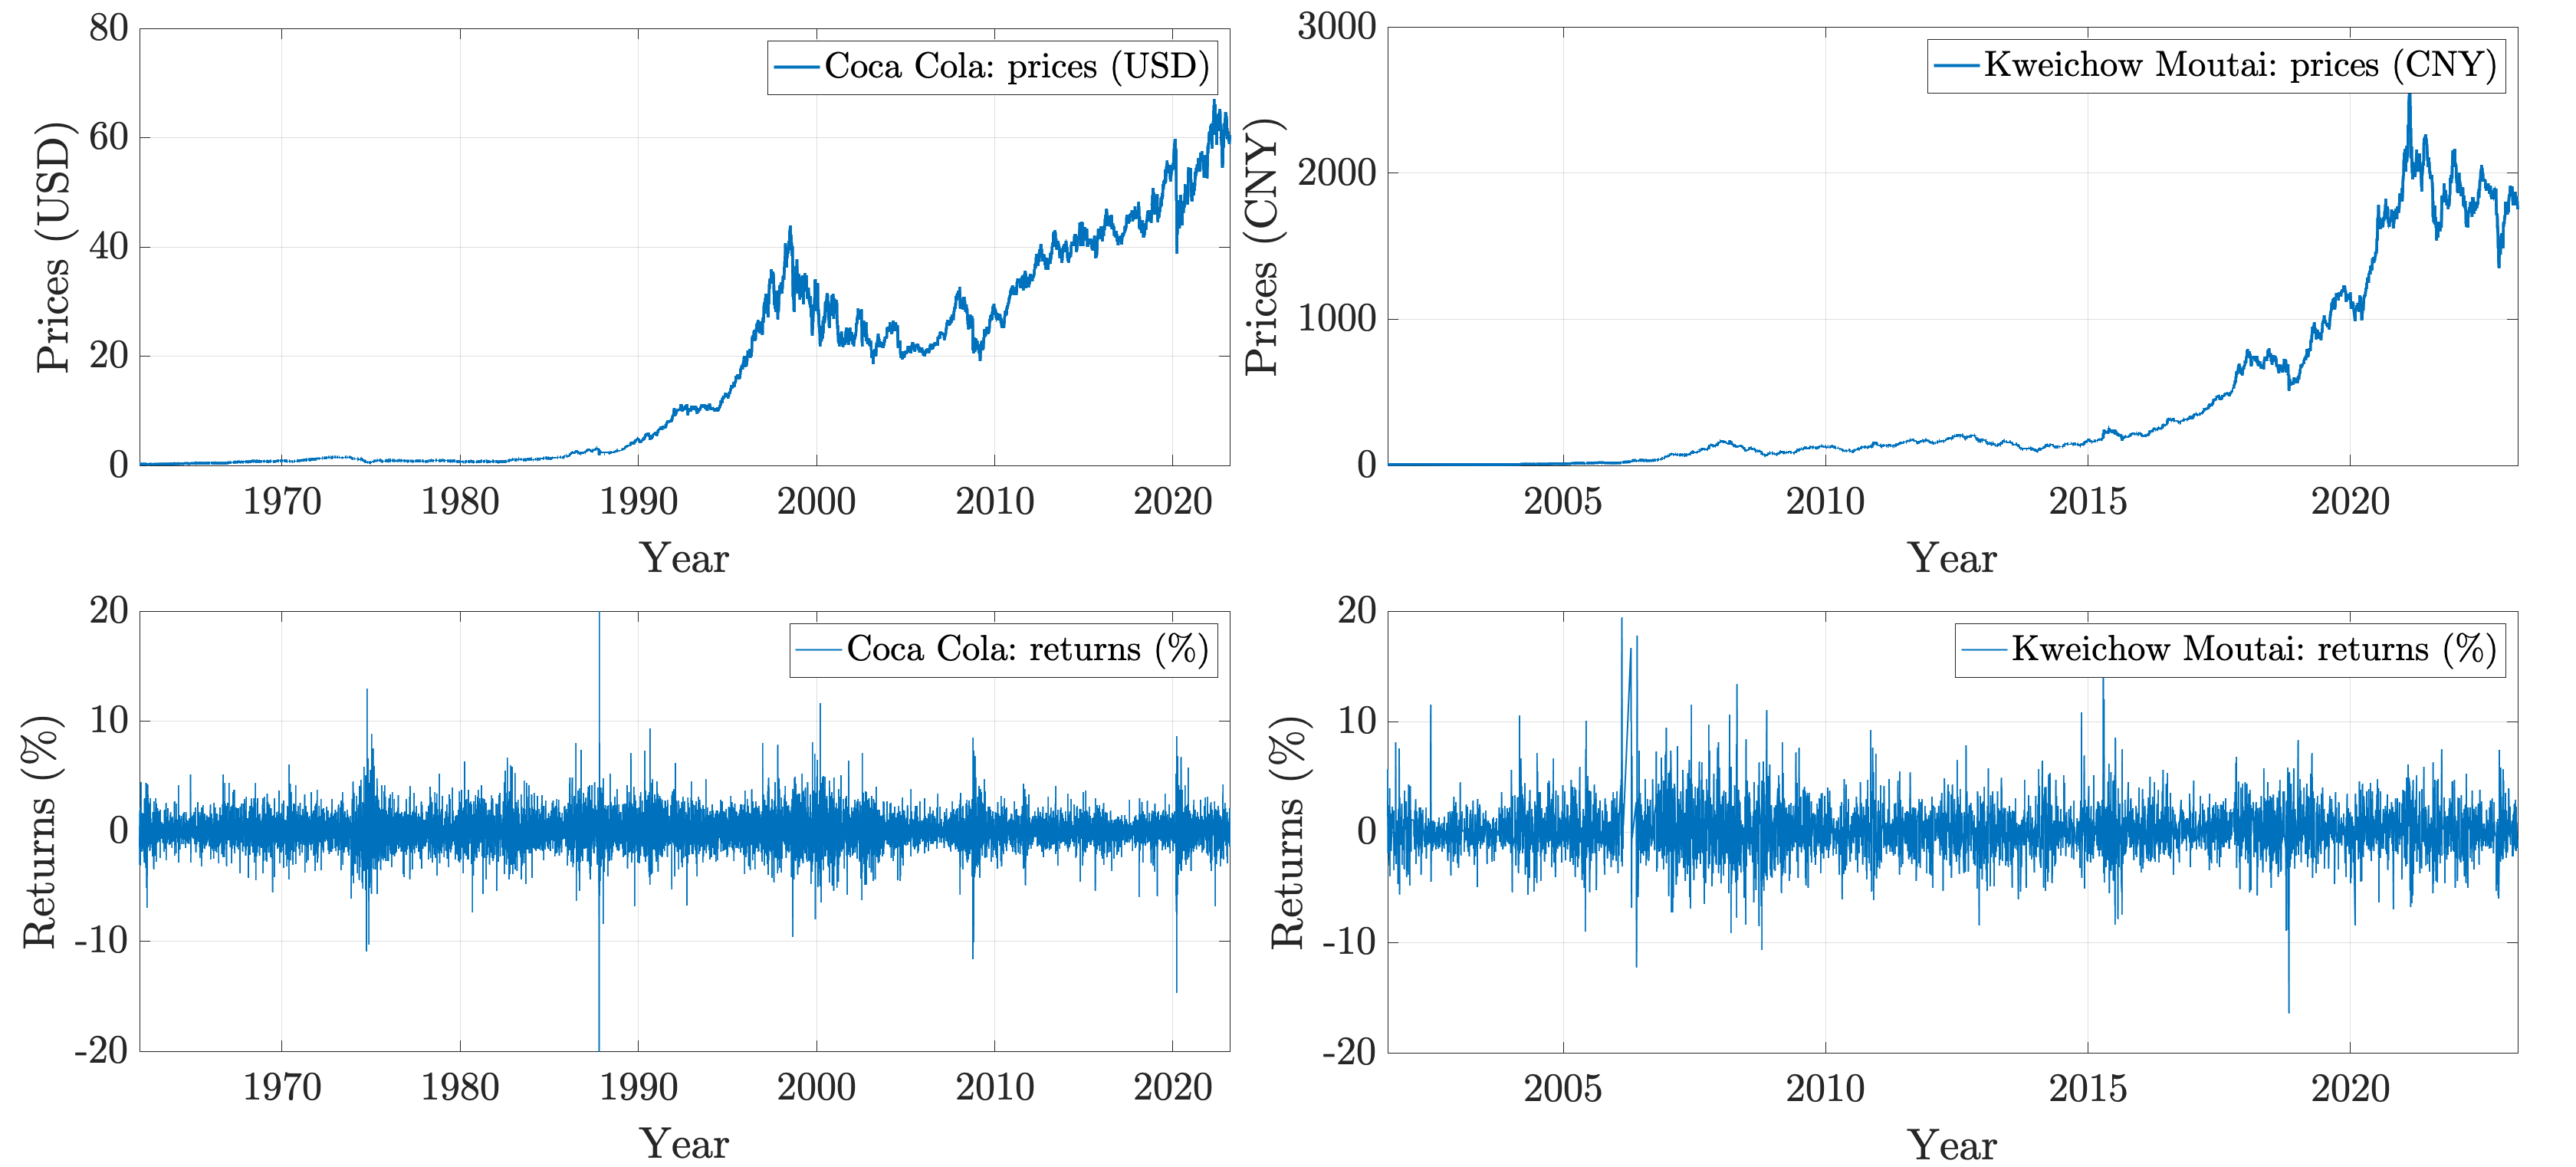
\includegraphics[width= 14cm]{visual_insight.png}
		\end{figure}
	\end{frame}

	\begin{frame}{Анализ данных (скалограмма) --- Coca Cola}
		\begin{figure}[H]
			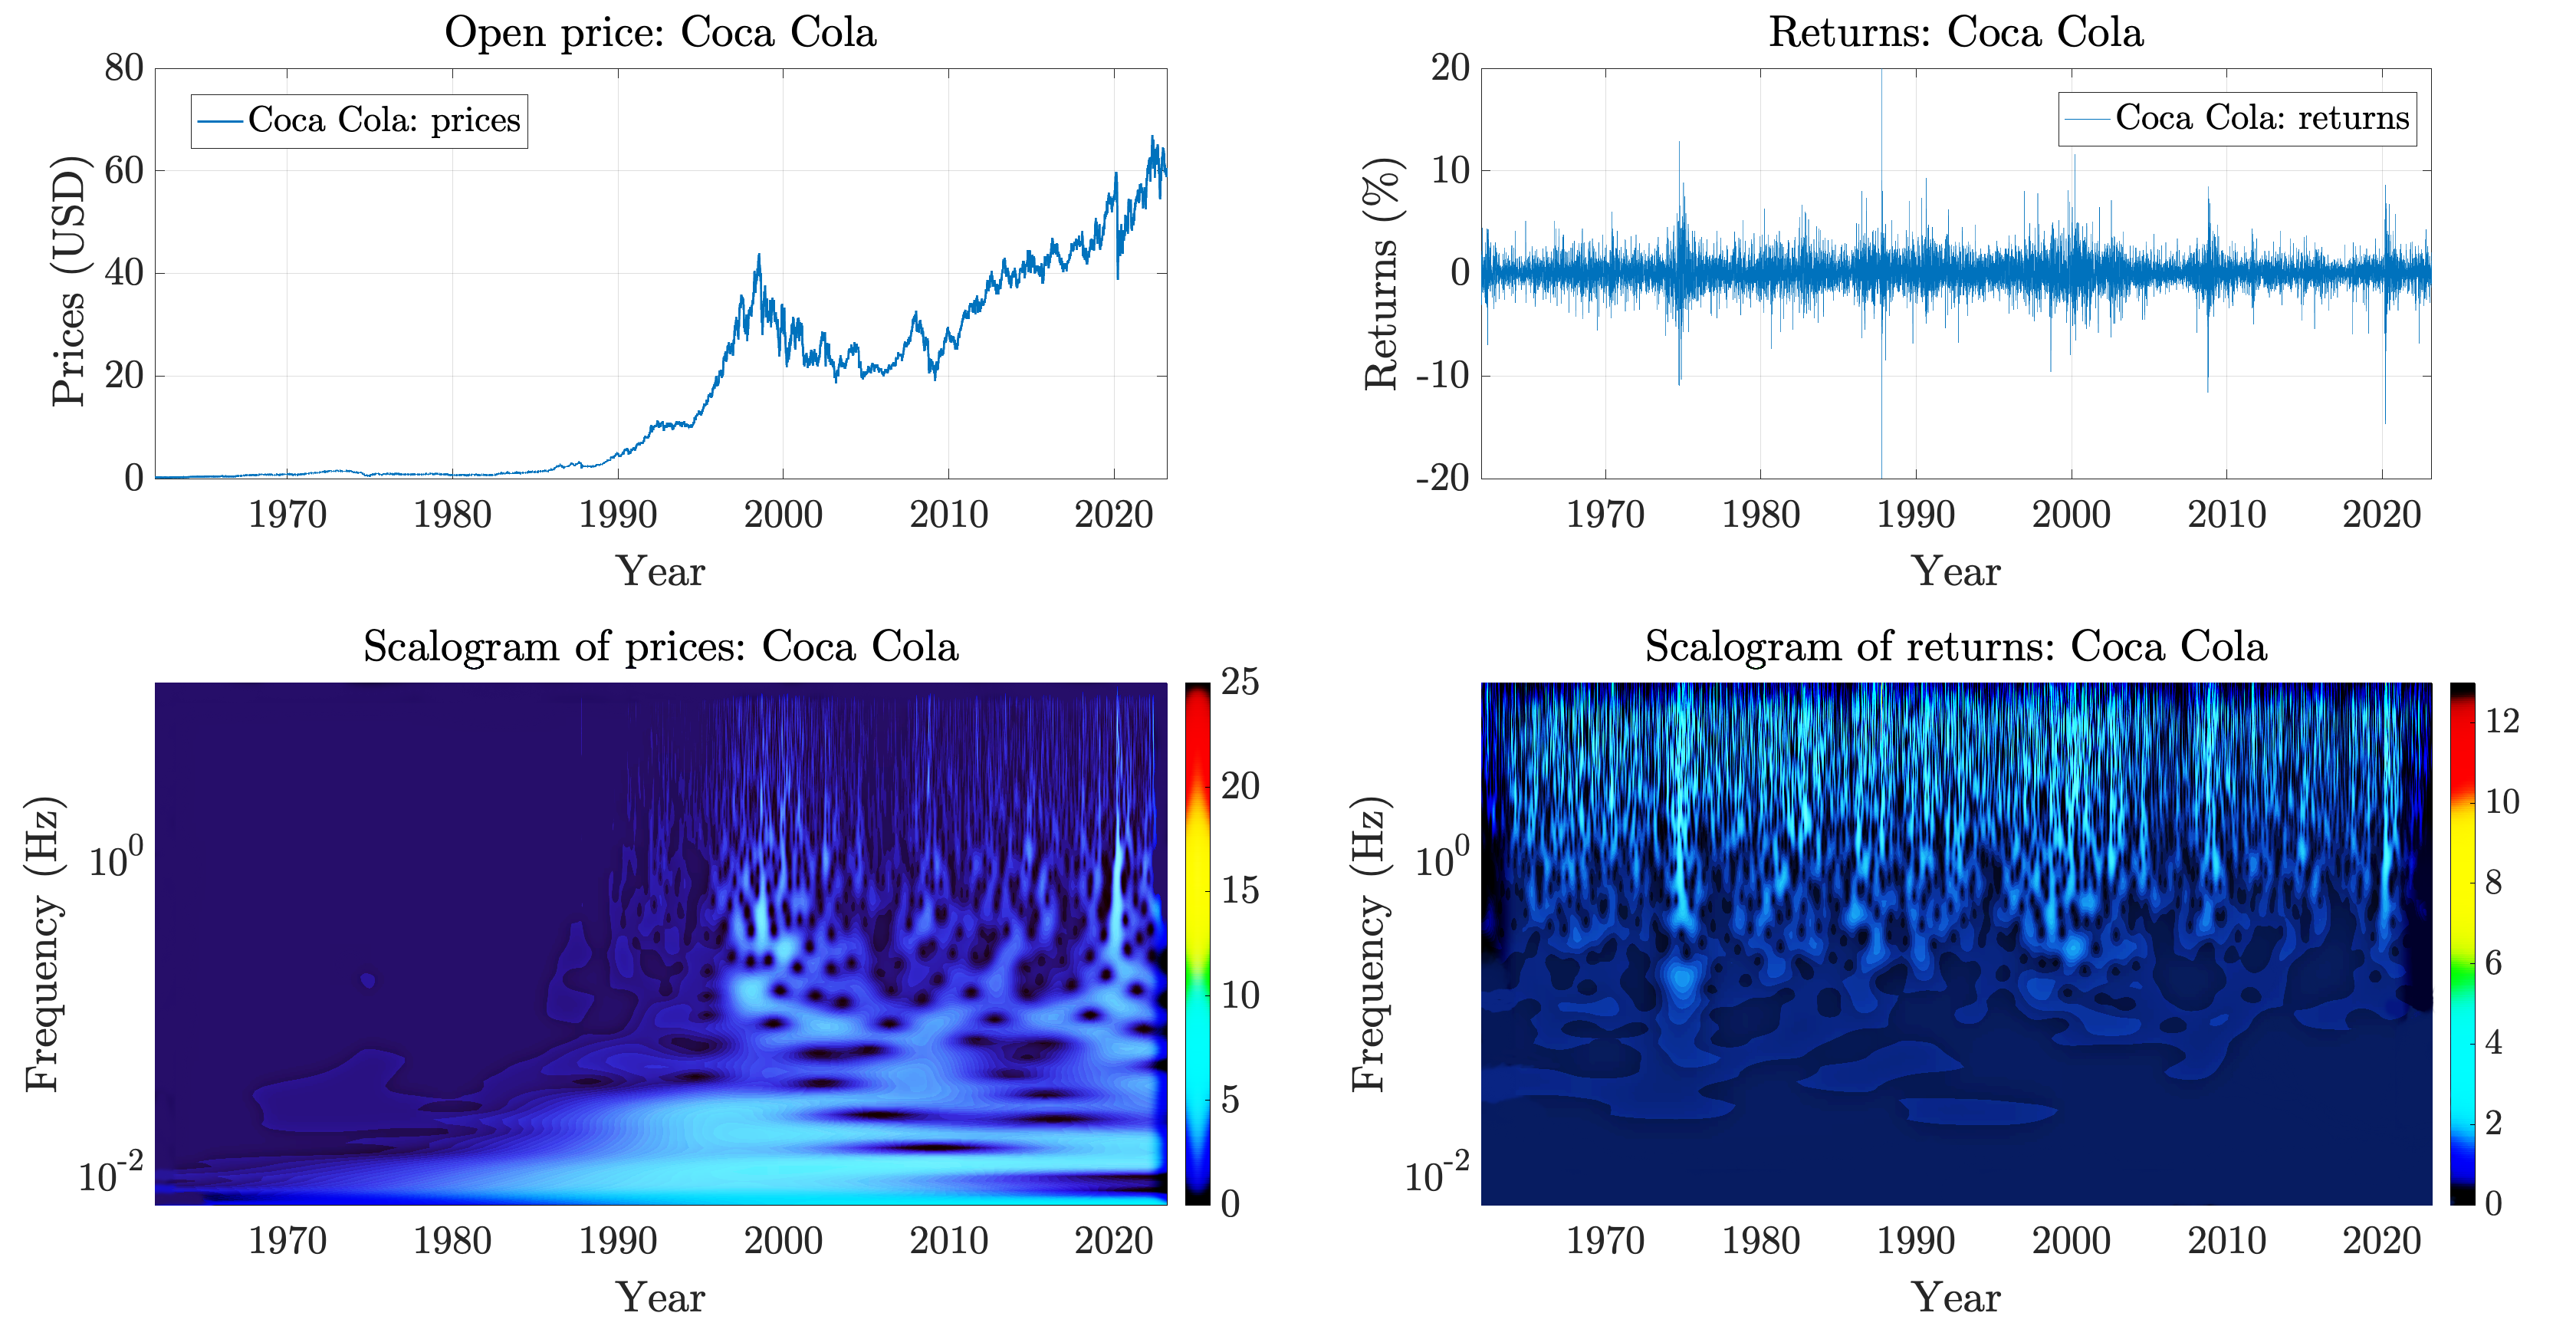
\includegraphics[width= 14cm]{scalogram_insights_us.png}
		\end{figure}
	\end{frame}

	\begin{frame}{Анализ данных (скалограмма) --- Kweichow Moutai}
		\begin{figure}[H]
			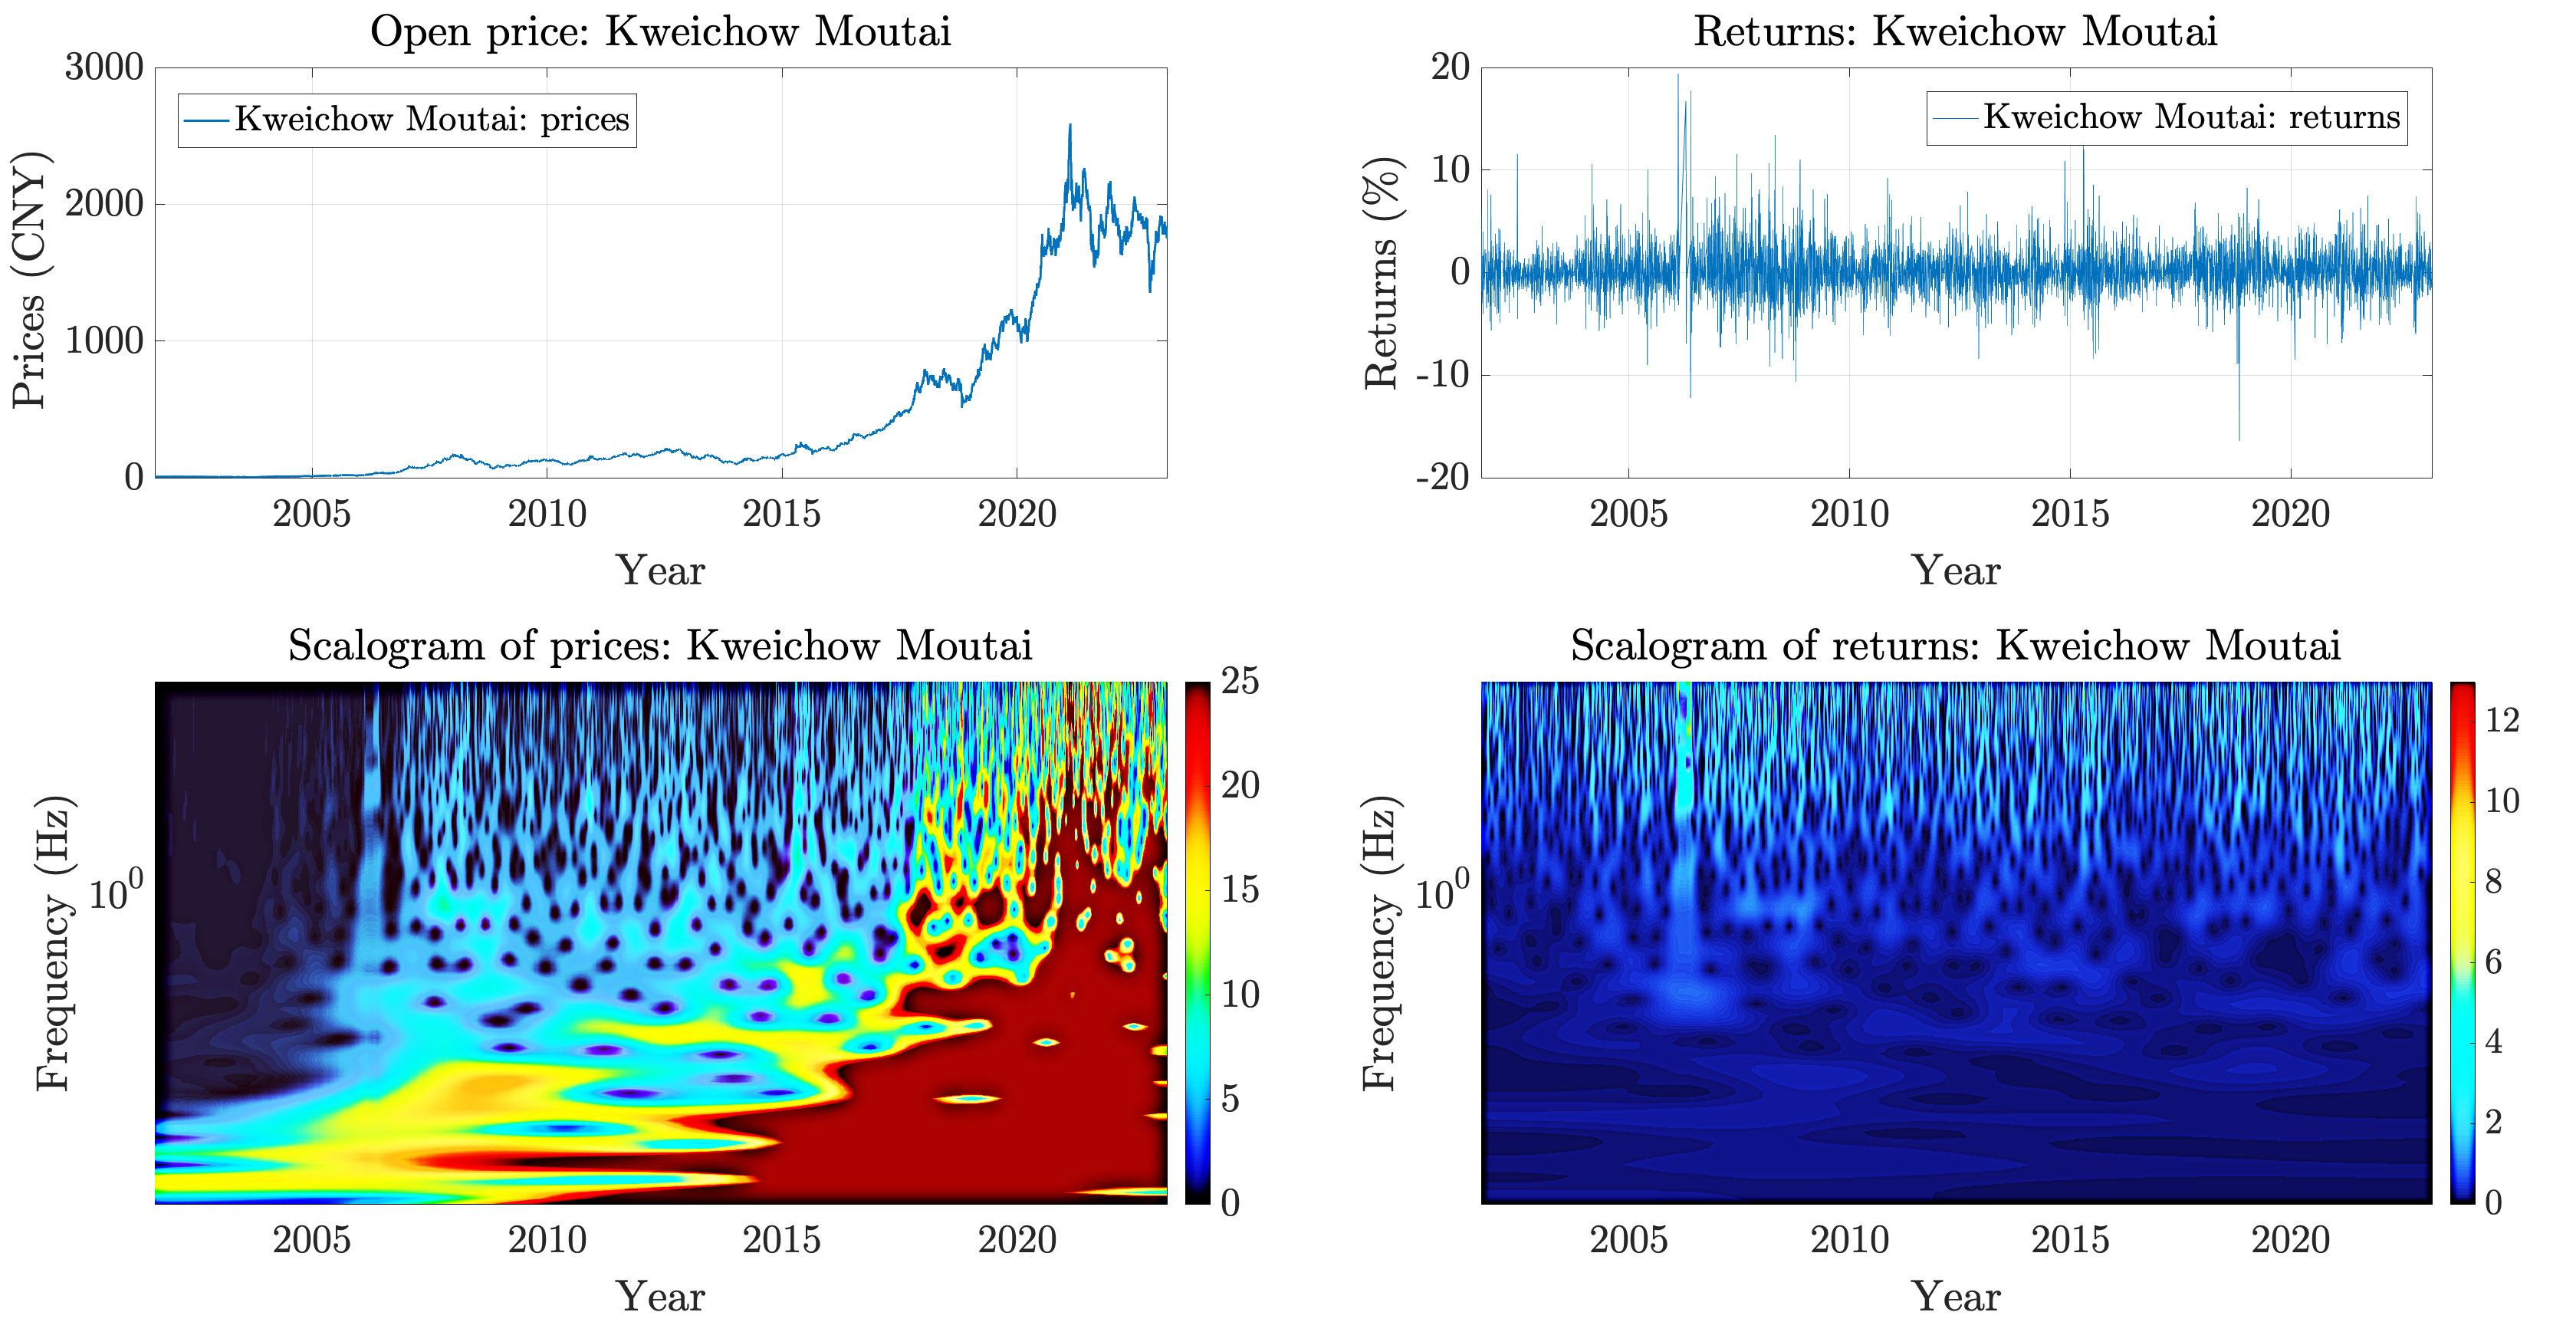
\includegraphics[width= 14cm]{scalogram_insights_china.png}
		\end{figure}
	\end{frame}

	
	\subsection{Метод (как доказываем?)}
	\begin{frame}{Метод}
		\begin{columns}
			\begin{column}{0.5\textwidth}
				\textbf{Эконометрический подход}:
				\begin{center}
					\begin{enumerate}
						\item EWMA
						\item ARIMA
						\item ARIMA + (FI)GARCH
						\item ARFIMA
						\item ARFIMA + (FI)GARCH
						\item SSA (Singular Spectrum Analysis)
					\end{enumerate}
				\end{center}
			\end{column}
			\hfill
			\begin{column}{0.5\textwidth}
				\textbf{Нейросетевой подход}:
				\begin{center}
					\begin{enumerate}
						\item MLP/RNN/WN
						\item MSSA/EWMA + MLP/RNN/WN
						\item No "transformers" $\Leftarrow$ \cite{zeng2022transformers}
					\end{enumerate}
				\end{center}
				\textbf{Топологическая функция}:
				\begin{equation}
					\text{WAPE}(\hat{y}, y) = \frac{\sum_{t= 1}^n |y_t - \hat{y}_t|}{\sum_{t= 1}^n |y_t|} \cdot 100\%
				\end{equation}
			\end{column}
		\end{columns}
		\vspace{1cm}
		(M)SSA --- Multistage Singular Spectrum Analysis \cite{kuang2020efficient}\\
		MLP --- Multilayer Perceptron \cite{rosenblatt1961principles}\\
		RNN --- Recurrent Neural Networks \cite{hochreiter1997long}\\
		WN --- Wavelet Network \cite{alexandridis2014wavelet}
	\end{frame}
	
	\section{Пост эксперимент}
	\subsection{Сравнительная диаграмма (результат)}
	\begin{frame}{Диаграмма WAPE отклонений прогнозов цен (\%)}
		\begin{figure}[H]
			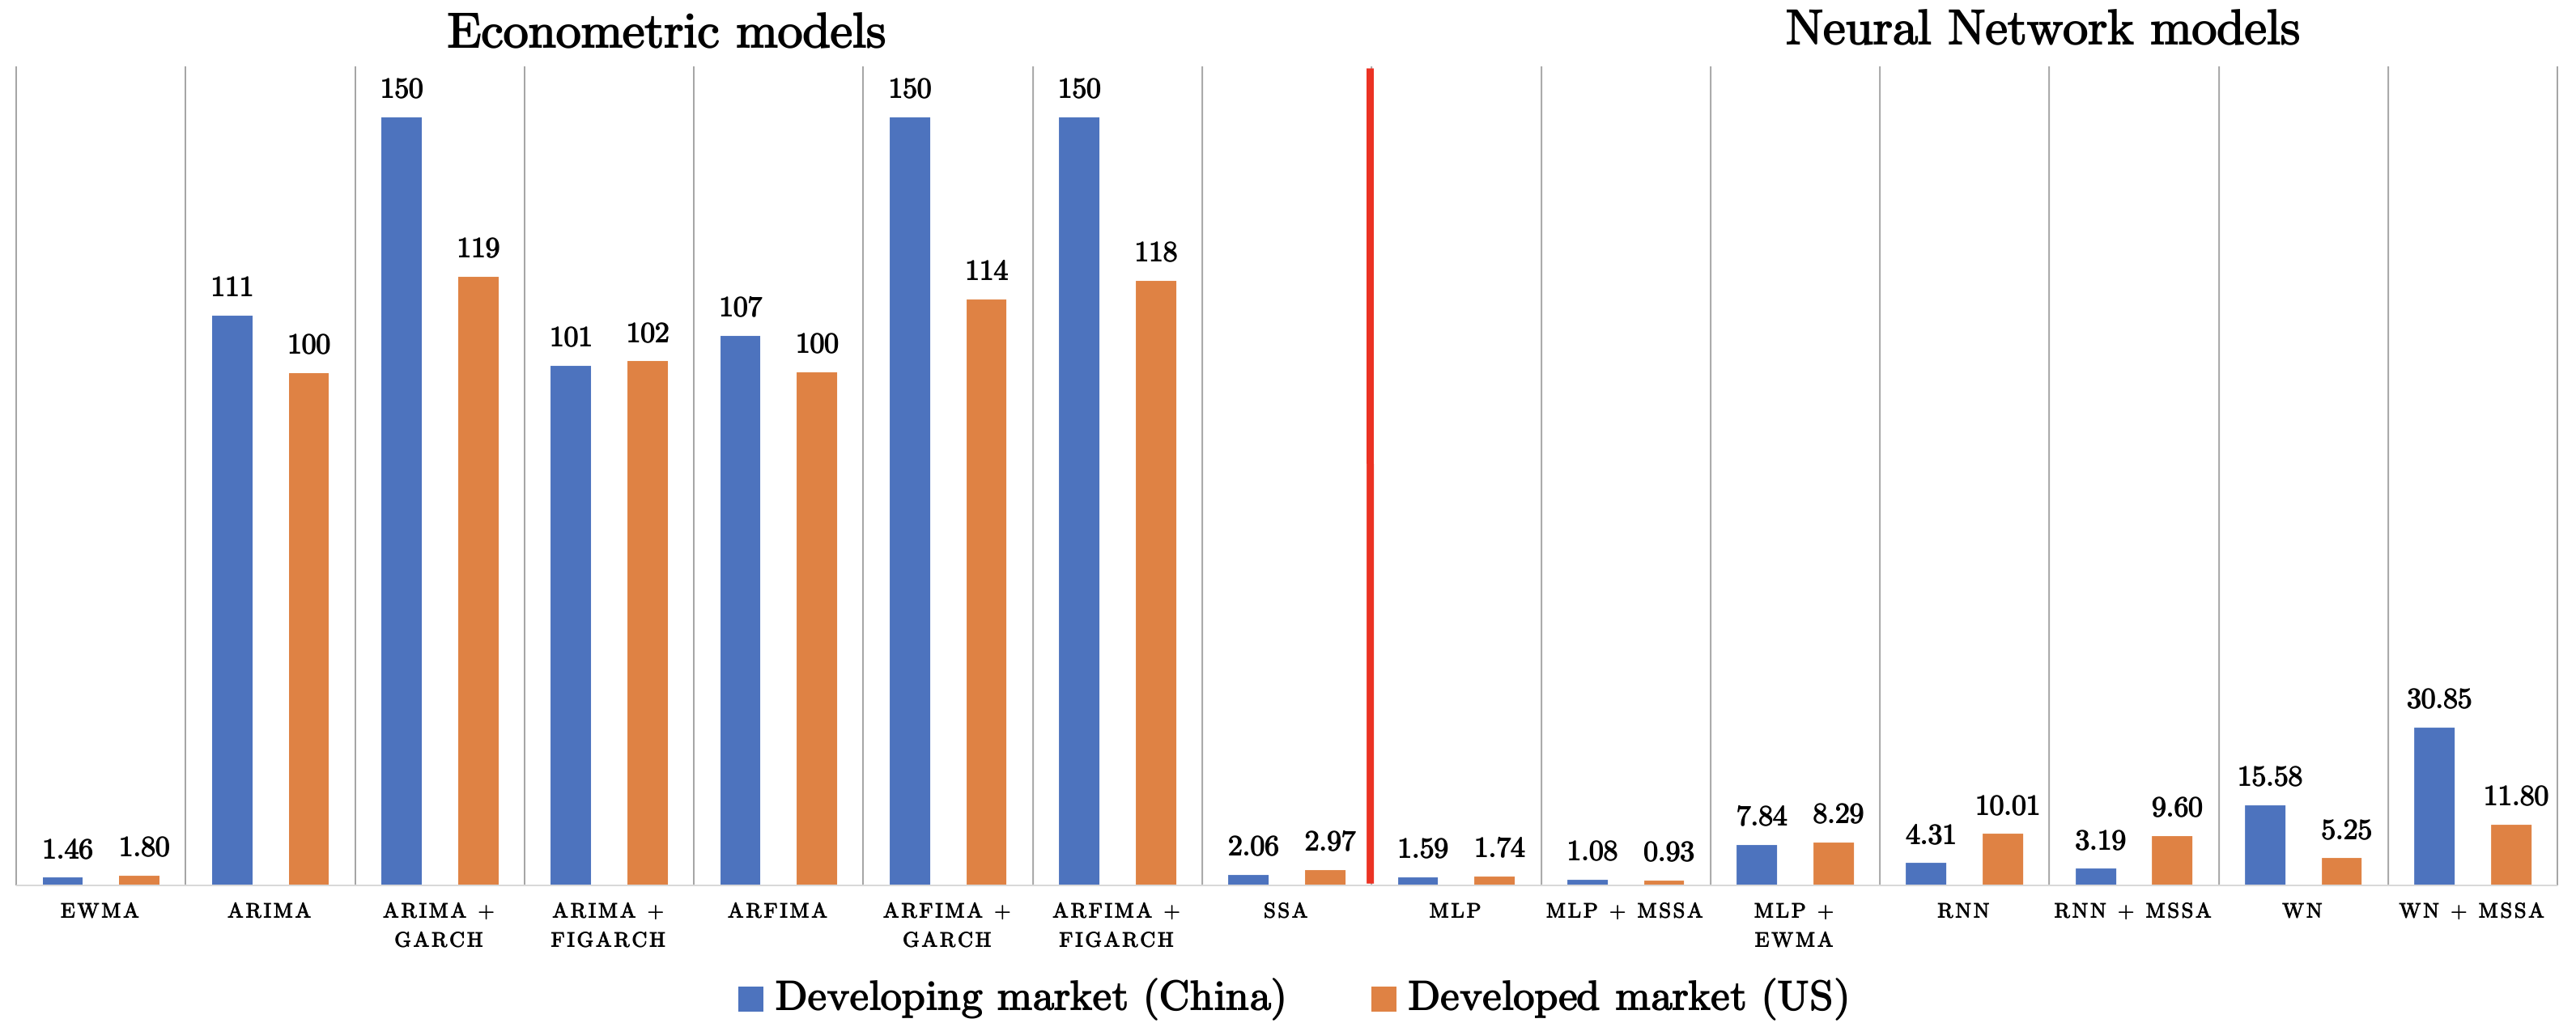
\includegraphics[width= 14cm]{table_prices.png}
		\end{figure}
	\end{frame}

	\begin{frame}{Диаграмма WAPE отклонений прогнозов доходностей (\%)}
		\begin{figure}[H]
			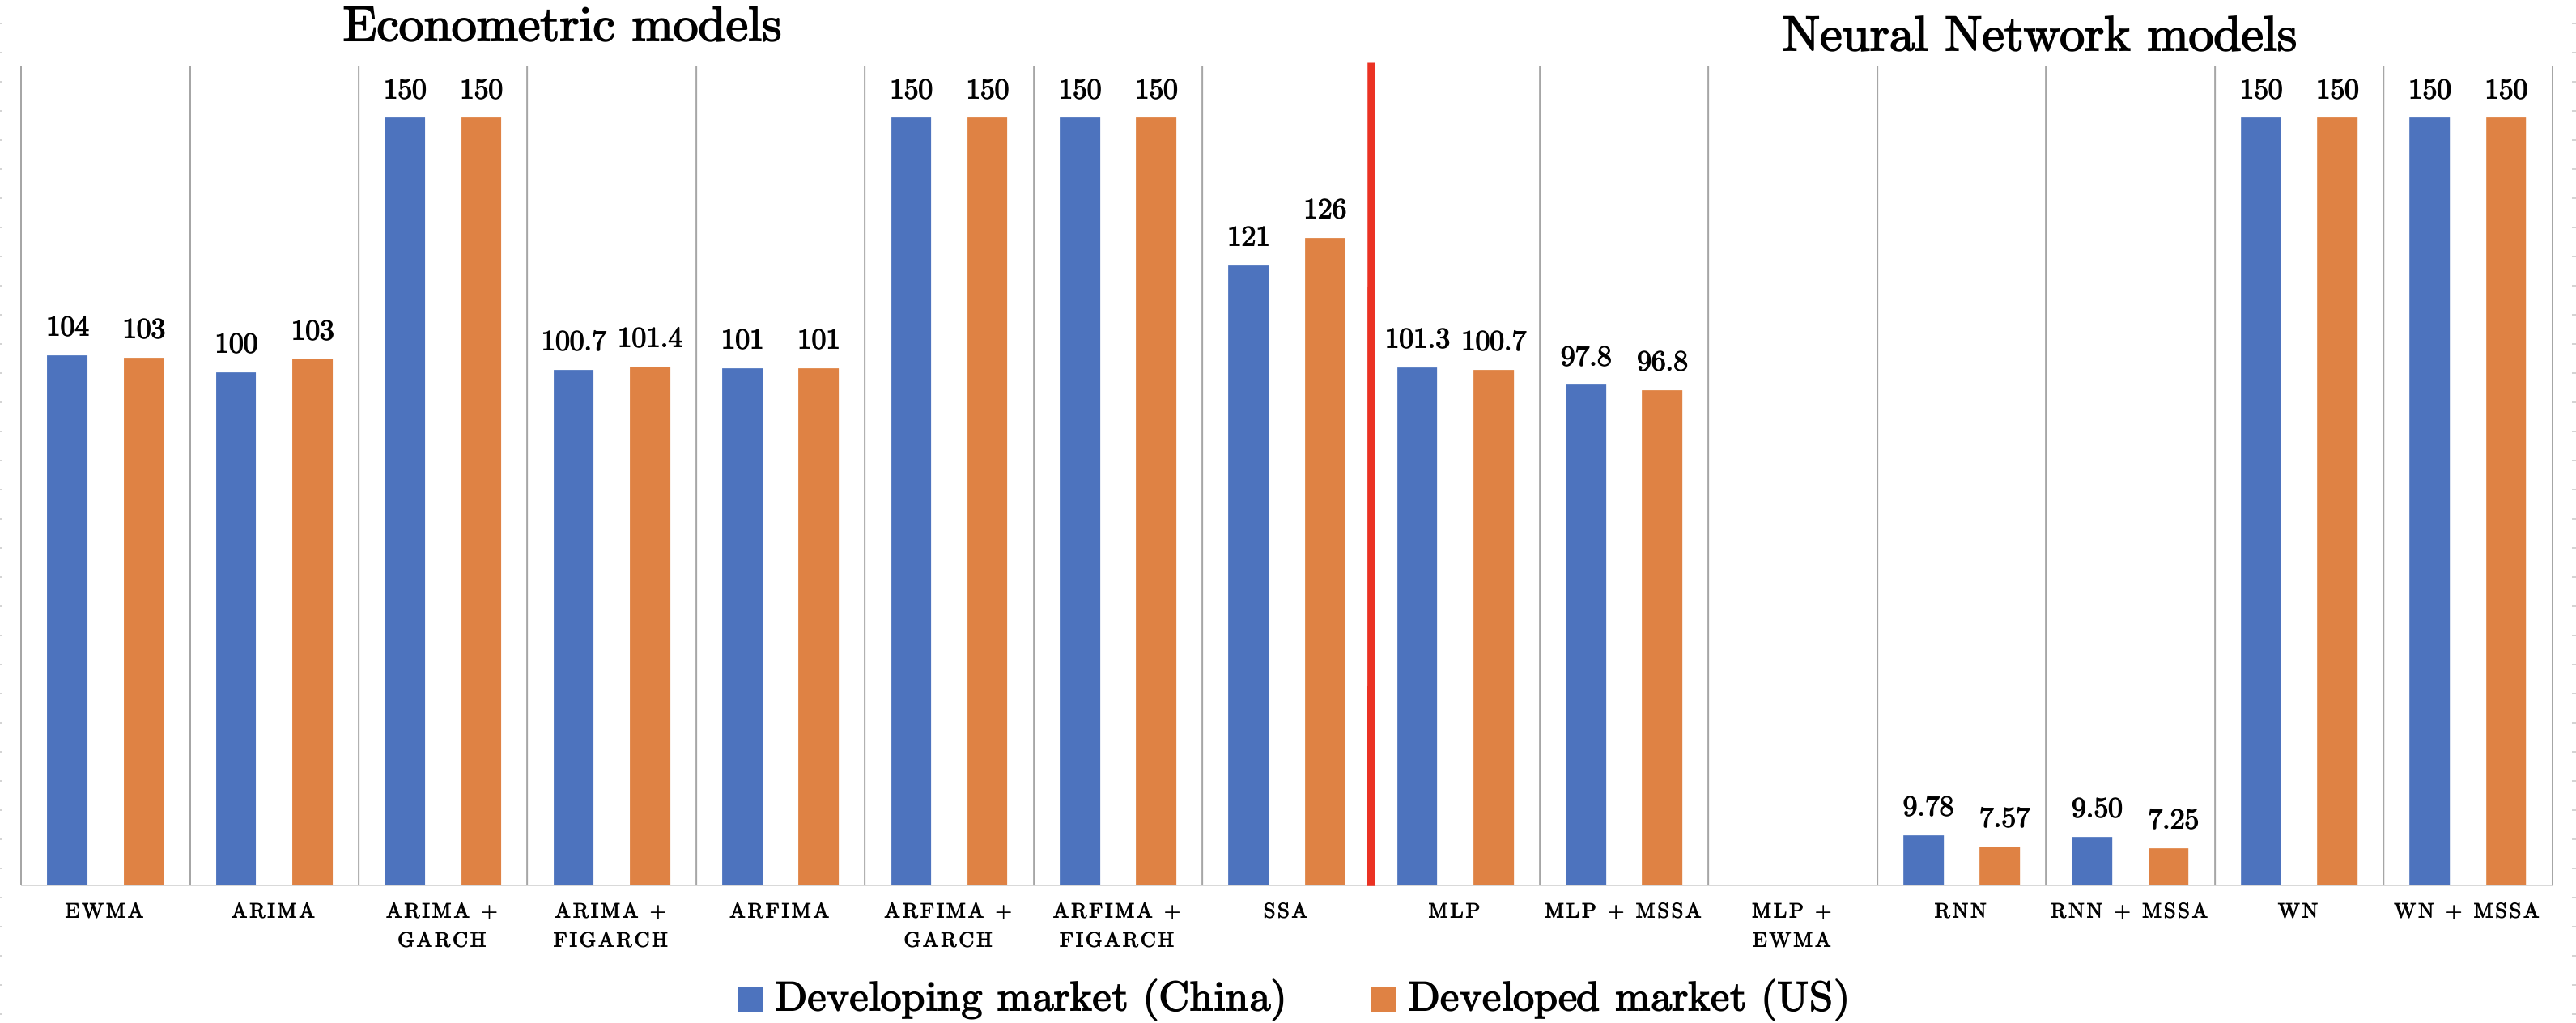
\includegraphics[width= 14cm]{table_returns.png}
		\end{figure}
	\end{frame}
	
	\subsection{Обсуждение (новые инсайды)}
	\begin{frame}{Обсуждение (новые инсайды)}
		\begin{enumerate}
			\item WAPE  для прогнозов цен $\ll$ WAPE для доходностей.
			\item MSSA + MLP лучшая для цен.
			\item MSSA + RNN лучшая для доходностей.
			\item Эконометрические модели плохи для прогнозов доходностей.
			\item Эконометрические модели менее точны для цен развивающихся рынков.
			\item (MSSA) Нет шума $\Rightarrow$ более точный прогноз: \textbf{исключение} Wavelet Networks.
			\item EWMA --- быстрый и хороший в точности статистический подход $\equiv$ trade off.
			\item Boosting вида ARIMA + GARCH, ARFIMA + GARCH --- плохой подход.
			\item ARFIMA лучше ARIMA $\Rightarrow$ рыночная фрактальность существует.
		\end{enumerate}
	\end{frame}
	
	\section{Ссылки}
	\begin{frame}[allowframebreaks]{Ссылки}
		\bibliographystyle{apalike}
		\bibliography{./source/bibliography/bibliography}
	\end{frame}
	
	\section{Заключение}
	\begin{frame}{Заключение}
		\begin{center}
			\LARGE
			Спасибо за внимание!
		\end{center}
	\end{frame}
\end{document}